\chapter{Постановка задачи}
\label{chapter1}

\section{Термины и понятия}

В данном разделе описаны термины, используемые других частях представленной работы. При этом смысл многих терминов сужен, по сравнению, с их обычным смыслом. Это связано, с тем, что данная работа ориентирована в первую очередь, разработку системы построения отчетов автотестов. В дальнейшем приведенные термины будут использоваться в указанных значениях, если не оговорено обратное.

\subsection{Тестирование}

{\bf Аттачмент (attachment)} ---
любая информация, например, скриншот или лог, которую надо сохранить вместе с результатами теста.  

{\bf История (user story, story)} ---
модуль, часть функциональности, из которых может состоять требование.

{\bf Контекст теста (test context, test fixture)} ---
все, что нужно тестируемой системе чтобы мы могли ее протестировать. Например, наглядно понятно, что такое контекст теста в тестовом фремворке RSpec:

\begin{itemize}
\item контекст --- множество фруктов содержащих = {яблоко, апельсин, грушу};
\item экспертиза --- удалим апельсин из множества фруктов;
\item проверка --- множество фруктов содержит = {яблоко, груша}.
\end{itemize}

{\bf Ошибка теста (test error)} ---
ошибка, возникающая в ходе выполнения теста. Например, ошибка может возникнуть в проверяемой системе, или в самом тесте. Также ошибка может возникнуть в окружении (например, в операционной системе, виртуальной машине). Как правило, ошибка в самом тесте, а не в проверяемой системе.

{\bf Падение теста (test failure)} ---
тест падает, когда в проверке утверждений актуальное значение не совпадает с ожидаемым. Обычно означает наличие ошибки в проверяемой системе.

{\bf Разработка через тестирование (TDD, test-driven development)} ---
техника разработки программного обеспечения, которая основывается на повторении очень которких циклов:

\begin{itemize}
\item написание теста на новую/изменяемую функциональность;
\item имплементация функциональности. Тест должен пройти;
\item рефакторинг кода под соответствующие стандарты разработки.
\end{itemize}

{\bf Разработка через требования (BDD, behavior-driven development)} ---
Разновидность разработки через тестирование, сфокусированная на тестах в которых четко описаны ожидаемые требования к тестируемой системе. Упор делается на то, что тесты используются как документация работы системы.

{\bf Результат теста (test result)} ---
тест, или тест суит могут быт ьзапущены несколько раз, и каждый раз возращать различные результаты проверок.

{\bf Тест} ---
некоторая процедура, котороая может быть выполена вручную или автоматически, и может быть использована для проверки ожидаемых требований к тестируемой системы. Тест часто называют тесткейсом.

{\bf Тест кейс (test case)} ---
обычно синоним для понятия "тест". В xUnit это также может обозначать тестовый класс, как месtex boldто в которое содержит тестовые методы.

{\bf Тест прошел (test success)} ---
ситуация, в которой проверка каждого утверждения в тесте прошла успешна (актуальные значения совпали с ожидаемыми), и в процессе выполенения теста не произошло никаких ошибок теста.

{\bf Тест ран (test run)} ---
запуск некоторого числа тестов или тестсуитов. После выполнения тестов из тестрана, мы можем получить их результаты.

{\bf Тест суит (test suite)} ---
способ наименования некоторого числа тестов, которые могут быть запущены вместе.

{\bf Тестируемая cистема (System Under Test)} ---
любая вещь, которую мы проверяем, например, метод, класс, объект, приложение.

{\bf Требование (feature)} ---
часть функциональности развивающейся системы, которая может быть протестирована.

{\bf Шаг (step)} ---
некоторая логическая часть теста. Каждый тест может состоять из одного или нескольких шагов. Как правило, шаги отображают сценарий теста.

{\bf Шаг теста (test step)} ---
смотри "Шаг".

{\bf xUnit} ---
под этим термином подразумевается любой член семейства инфраструктур автоматизации тестов (Test Automation Framework), применяемых для автоматизации созданных вручную сценариев тестов. Для большинства современных языков программирования существует как минимум одна реализация xUnit. Обычно для автоматизации применяется тот же язык, который использовался для написания тестируемой ситстемы. Хотя это не всегда так, использовать подобную стратегию проще, поскольку тесты легко получают доступ к программному интерфейсу тестируемой системы.

{\bf WebDriver} ---
утилита, позволяющая эмулировать действия пользователя в различных браузерах.

Большинство членов xUnit реализованы с использованием объектно-ориентированной парадигмы.

\subsection{Сокращения}

{\bf SUT} --- System Under Test, смотри "Тестируемая система".

\section{Обоснование актуальности}

На данный момент, практически отсутствуют системы, которые позволяют решать поставленную задачу. Для xUnit тестов можно построить стандартный отчет, но он подходит только для модульного тестирования, то есть в нем нет возможности сохранения дополнительной информации о ходе теста, сценария теста. Также у некоторых тестовых фремворков есть свои отчеты (например, Thucydides), но они узконаправленные, и позволяют действовать только в рамках соответсвующих фремворков. Для большинства членов семейства xUnit систем построения отчетов, кроме стандартного, нет.

Из-за отстутствия универсального решения, и наличия большого числа высокоуровневых тестов, анализ результатов отнимает очень много времени и сил. И часто узкое причина длинного цикла разработки именно затянувшийся процесс тестирования.

\section{Обзор существующих систем}

\subsection{Surefire}
Семейство xUnit предлагает стандартный отчет, который называется surefire. Это простой отчет, содержащий список тестов, и для каждого теста информацию о его статусе, времени работы и сообщения об ошибке (если имеется). Данное решение подходит для анализа результатов модульных тестов, но не годиться в рамках поставленной задачи.

\subsection{Thucydides}
Thucydides --- тестовый фремворк на основе jUnit. Он предоставляет возможность писать WebDriver'ные тесты, есть возможность разбивать тесты на шаги, и сохранять скриншоты. Основным недостатоком данной системы является то, что она слишком узконаправленная, и накладывает слишком много ограничений на как тесты и тестируемые системы. 

\section{Технический и организационный контекст}
Рассмотрим структуру разработки системы отчетов автотестов. Автор работы является основным разработчиком фремворка (Allure), активно взаимодействует с остальными участниками разработки. Основным заказчиком является отдел тестирования компании Яндекс, в лице Ерошенко Артема Михайловича, который также является основным идейным вдохновителем и руководителем разработки. 

Первый прототип, а так же первые две версии были спроектированы и разработаны автором данной работы, совмество с Артемом Михайловичем. Дальше к разработке присоеденился профессиональный front-end разработчик Сердюк Борис Дмитриевич, который переработал "морду" отчета, и до сих пор активно участвует в поддержке и развитии фреймворка. 

Изначально перед автором стояла задача предложить структуру фремворка, разработать прототип и адаптировать фремворк под работу с jUnit и pyTest. 

Общую схему работы фреймворка можно увидеть на рисунке \ref{fig:allure}.

\begin{figure}[htb]
\centering
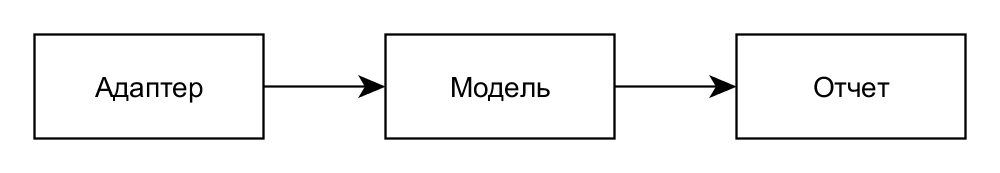
\includegraphics[height=30mm]{allure.png}
\caption{Общая схема работы Allure}
\label{fig:allure}
\end{figure}

Фактически, работа фремворка состоит из двух частей. Сначала надо собрать данные о ходе выполнения тестов, а затем сгенерировать из них отчет. 

\section{Уточненные требования к работе}

Обобщая вышесказанное, выведем следующие основные цели данной работы:

\begin{itemize}
\item разработать систему, позволяющую собирать дополнительную информацию о теста и отображать ее в виде отчета:
\begin{itemize}
\item система должна легко подключаться к большому числу уже написанных тестов;
\item система должна легко адаптироваться под разные языки программирования;
\item система должна быть модульной, легко расширяться;
\end{itemize}
\item написать первый прототип системы;
\item реализовать первую версию программы;
\item протестировать систему в реальных условиях;
\item проанализировать результаты работы системы.
\end{itemize}

Результатом данной работы будет являться готовый роботоспособный фремворк, активно используемый в тестировании в качестве универсального способа
отображения результатов работы автотестов.
